\PassOptionsToPackage{unicode=true}{hyperref} % options for packages loaded elsewhere
\PassOptionsToPackage{hyphens}{url}
%
\documentclass[man]{apa6}
\usepackage{lmodern}
\usepackage{amssymb,amsmath}
\usepackage{ifxetex,ifluatex}
\usepackage{fixltx2e} % provides \textsubscript
\ifnum 0\ifxetex 1\fi\ifluatex 1\fi=0 % if pdftex
  \usepackage[T1]{fontenc}
  \usepackage[utf8]{inputenc}
  \usepackage{textcomp} % provides euro and other symbols
\else % if luatex or xelatex
  \usepackage{unicode-math}
  \defaultfontfeatures{Ligatures=TeX,Scale=MatchLowercase}
\fi
% use upquote if available, for straight quotes in verbatim environments
\IfFileExists{upquote.sty}{\usepackage{upquote}}{}
% use microtype if available
\IfFileExists{microtype.sty}{%
\usepackage[]{microtype}
\UseMicrotypeSet[protrusion]{basicmath} % disable protrusion for tt fonts
}{}
\IfFileExists{parskip.sty}{%
\usepackage{parskip}
}{% else
\setlength{\parindent}{0pt}
\setlength{\parskip}{6pt plus 2pt minus 1pt}
}
\usepackage{hyperref}
\hypersetup{
            pdftitle={Decisions Decisions Decisions: Carrying out Latent Profile Analysis in Accordance With Best Practices Using the tidyLPA R package},
            pdfauthor={Joshua Rosenberg, Caspar van Lissa, Jennifer Schmidt, Patrick Beymer, Daniel Anderson, \& Matthew Schell},
            pdfkeywords={Latent Profile Analysis, mixture models, finite mixture models, tutorial, R, MPlus, mclust},
            pdfborder={0 0 0},
            breaklinks=true}
\urlstyle{same}  % don't use monospace font for urls
\usepackage{color}
\usepackage{fancyvrb}
\newcommand{\VerbBar}{|}
\newcommand{\VERB}{\Verb[commandchars=\\\{\}]}
\DefineVerbatimEnvironment{Highlighting}{Verbatim}{commandchars=\\\{\}}
% Add ',fontsize=\small' for more characters per line
\usepackage{framed}
\definecolor{shadecolor}{RGB}{248,248,248}
\newenvironment{Shaded}{\begin{snugshade}}{\end{snugshade}}
\newcommand{\AlertTok}[1]{\textcolor[rgb]{0.94,0.16,0.16}{#1}}
\newcommand{\AnnotationTok}[1]{\textcolor[rgb]{0.56,0.35,0.01}{\textbf{\textit{#1}}}}
\newcommand{\AttributeTok}[1]{\textcolor[rgb]{0.77,0.63,0.00}{#1}}
\newcommand{\BaseNTok}[1]{\textcolor[rgb]{0.00,0.00,0.81}{#1}}
\newcommand{\BuiltInTok}[1]{#1}
\newcommand{\CharTok}[1]{\textcolor[rgb]{0.31,0.60,0.02}{#1}}
\newcommand{\CommentTok}[1]{\textcolor[rgb]{0.56,0.35,0.01}{\textit{#1}}}
\newcommand{\CommentVarTok}[1]{\textcolor[rgb]{0.56,0.35,0.01}{\textbf{\textit{#1}}}}
\newcommand{\ConstantTok}[1]{\textcolor[rgb]{0.00,0.00,0.00}{#1}}
\newcommand{\ControlFlowTok}[1]{\textcolor[rgb]{0.13,0.29,0.53}{\textbf{#1}}}
\newcommand{\DataTypeTok}[1]{\textcolor[rgb]{0.13,0.29,0.53}{#1}}
\newcommand{\DecValTok}[1]{\textcolor[rgb]{0.00,0.00,0.81}{#1}}
\newcommand{\DocumentationTok}[1]{\textcolor[rgb]{0.56,0.35,0.01}{\textbf{\textit{#1}}}}
\newcommand{\ErrorTok}[1]{\textcolor[rgb]{0.64,0.00,0.00}{\textbf{#1}}}
\newcommand{\ExtensionTok}[1]{#1}
\newcommand{\FloatTok}[1]{\textcolor[rgb]{0.00,0.00,0.81}{#1}}
\newcommand{\FunctionTok}[1]{\textcolor[rgb]{0.00,0.00,0.00}{#1}}
\newcommand{\ImportTok}[1]{#1}
\newcommand{\InformationTok}[1]{\textcolor[rgb]{0.56,0.35,0.01}{\textbf{\textit{#1}}}}
\newcommand{\KeywordTok}[1]{\textcolor[rgb]{0.13,0.29,0.53}{\textbf{#1}}}
\newcommand{\NormalTok}[1]{#1}
\newcommand{\OperatorTok}[1]{\textcolor[rgb]{0.81,0.36,0.00}{\textbf{#1}}}
\newcommand{\OtherTok}[1]{\textcolor[rgb]{0.56,0.35,0.01}{#1}}
\newcommand{\PreprocessorTok}[1]{\textcolor[rgb]{0.56,0.35,0.01}{\textit{#1}}}
\newcommand{\RegionMarkerTok}[1]{#1}
\newcommand{\SpecialCharTok}[1]{\textcolor[rgb]{0.00,0.00,0.00}{#1}}
\newcommand{\SpecialStringTok}[1]{\textcolor[rgb]{0.31,0.60,0.02}{#1}}
\newcommand{\StringTok}[1]{\textcolor[rgb]{0.31,0.60,0.02}{#1}}
\newcommand{\VariableTok}[1]{\textcolor[rgb]{0.00,0.00,0.00}{#1}}
\newcommand{\VerbatimStringTok}[1]{\textcolor[rgb]{0.31,0.60,0.02}{#1}}
\newcommand{\WarningTok}[1]{\textcolor[rgb]{0.56,0.35,0.01}{\textbf{\textit{#1}}}}
\usepackage{graphicx,grffile}
\makeatletter
\def\maxwidth{\ifdim\Gin@nat@width>\linewidth\linewidth\else\Gin@nat@width\fi}
\def\maxheight{\ifdim\Gin@nat@height>\textheight\textheight\else\Gin@nat@height\fi}
\makeatother
% Scale images if necessary, so that they will not overflow the page
% margins by default, and it is still possible to overwrite the defaults
% using explicit options in \includegraphics[width, height, ...]{}
\setkeys{Gin}{width=\maxwidth,height=\maxheight,keepaspectratio}
\setlength{\emergencystretch}{3em}  % prevent overfull lines
\providecommand{\tightlist}{%
  \setlength{\itemsep}{0pt}\setlength{\parskip}{0pt}}
\setcounter{secnumdepth}{0}
% Redefines (sub)paragraphs to behave more like sections
\ifx\paragraph\undefined\else
\let\oldparagraph\paragraph
\renewcommand{\paragraph}[1]{\oldparagraph{#1}\mbox{}}
\fi
\ifx\subparagraph\undefined\else
\let\oldsubparagraph\subparagraph
\renewcommand{\subparagraph}[1]{\oldsubparagraph{#1}\mbox{}}
\fi

% set default figure placement to htbp
\makeatletter
\def\fps@figure{htbp}
\makeatother

\shorttitle{LPA Best Practices}
\affiliation{
\vspace{0.5cm}
\textsuperscript{1} University of Tennessee, Knoxville\\\textsuperscript{2} Utrecht University\\\textsuperscript{3} Michigan State University\\\textsuperscript{3} University of Oregon\\\textsuperscript{4} University of Wisconsin, Madison}
\keywords{Latent Profile Analysis, mixture models, finite mixture models, tutorial, R, MPlus, mclust\newline\indent Word count: suggested to be no more than 3,000}
\usepackage{csquotes}
\usepackage{upgreek}
\captionsetup{font=singlespacing,justification=justified}

\usepackage{longtable}
\usepackage{lscape}
\usepackage{multirow}
\usepackage{tabularx}
\usepackage[flushleft]{threeparttable}
\usepackage{threeparttablex}

\newenvironment{lltable}{\begin{landscape}\begin{center}\begin{ThreePartTable}}{\end{ThreePartTable}\end{center}\end{landscape}}

\makeatletter
\newcommand\LastLTentrywidth{1em}
\newlength\longtablewidth
\setlength{\longtablewidth}{1in}
\newcommand{\getlongtablewidth}{\begingroup \ifcsname LT@\roman{LT@tables}\endcsname \global\longtablewidth=0pt \renewcommand{\LT@entry}[2]{\global\advance\longtablewidth by ##2\relax\gdef\LastLTentrywidth{##2}}\@nameuse{LT@\roman{LT@tables}} \fi \endgroup}


\DeclareDelayedFloatFlavor{ThreePartTable}{table}
\DeclareDelayedFloatFlavor{lltable}{table}
\DeclareDelayedFloatFlavor*{longtable}{table}
\makeatletter
\renewcommand{\efloat@iwrite}[1]{\immediate\expandafter\protected@write\csname efloat@post#1\endcsname{}}
\makeatother

\title{Decisions Decisions Decisions: Carrying out Latent Profile Analysis in Accordance With Best Practices Using the tidyLPA R package}
\author{Joshua Rosenberg\textsuperscript{1}, Caspar van Lissa\textsuperscript{2}, Jennifer Schmidt\textsuperscript{3}, Patrick Beymer\textsuperscript{5}, Daniel Anderson\textsuperscript{4}, \& Matthew Schell\textsuperscript{3}}
\date{}

\authornote{

Correspondence concerning this article should be addressed to Joshua Rosenberg, 1122 Volunteer Blvd., Knoxville, TN, 37996. E-mail: \href{mailto:jmrosenberg@utk.edu}{\nolinkurl{jmrosenberg@utk.edu}}}

\abstract{

}

\begin{document}
\maketitle

\hypertarget{introduction}{%
\section{Introduction}\label{introduction}}

In statistics classes, textbooks, and workshops, an example like the following
is common:

\begin{quote}
Grades are normally distributed, with \(\mu\) = 75, \(\sigma\) = 5.
\end{quote}

Is there one distribution?

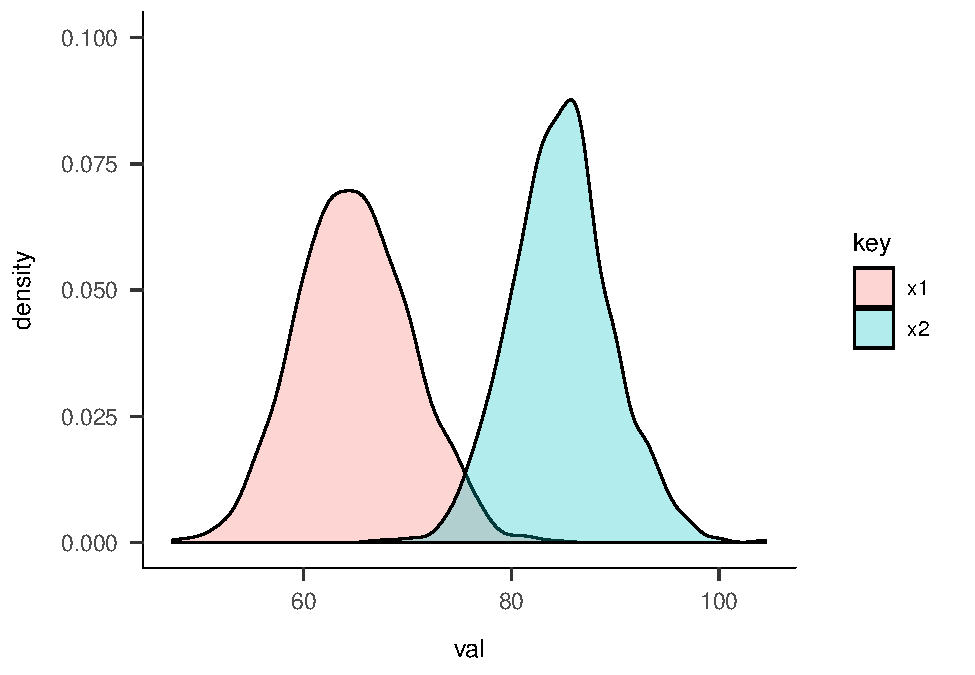
\includegraphics{paper_files/figure-latex/unnamed-chunk-2-1.pdf}

Or, are there two?

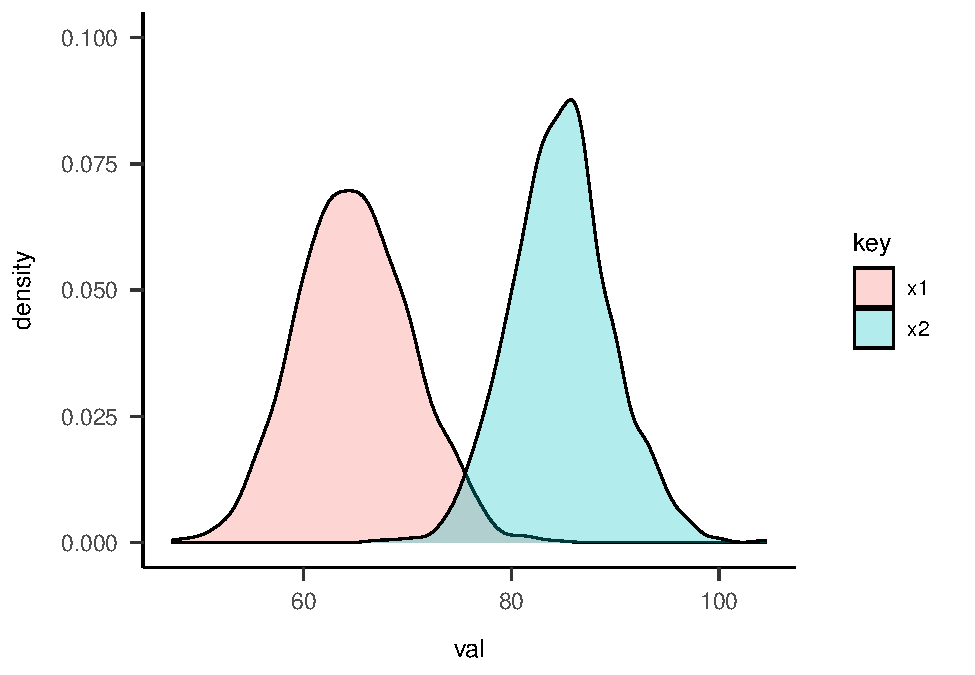
\includegraphics{paper_files/figure-latex/unnamed-chunk-3-1.pdf}

This kind of distribution (one that is \emph{bimodal}) is not exclusive to grades.
For teachers, psychologists, researchers, and even friends and family members,
people are highly-complex and not easily able to be characterized by \emph{one}
characteristic or personality trait--and its distribution.

In the social sciences, broadly, and in the psychological sciences, in
particular, a statistical method that can be used to describe how people, in
their individual particularities, may have similarities on the basis of some set
of measures through which they can be grouped in meaningful, distinctive ways.

This approach, which we view as having a provenance in developmental (or
\emph{person-oriented}) approaches (Bergman \& El-Khouri, 1997; Magnusson \&
Cairns, 1996; see Linnenbrink-Garcia \& Wormington, 2017, for a recent review) is
an example of a general mixture model (Harring \& Hodis, 2016; Pastor, Barron,
Miller, \& Davis, 2007).

In this tutorial, we aim to describe one of the most commonly-used---and
relevant to psychologists---application of the general mixture model, to cases
for which all of the variables for which (relatively) homogeneous groups are
identified from among a (relatively) heterogeneous sample are continuos, \emph{latent
profile analysis} (LPA). After describing the method and some examples of its
use, we provide a tutorial for carrying out LPA in the context of a
freely-available, open-source statistical software package that we have
developed and supported over the past three years for R (R Core Team, 2019),
tidyLPA. Finally, we offer some ideas about best practices and informed
recommendations for researchers aiming to use LPA in their applied work, and
conclude with reflections on the role of statistical software--especially
software that is freely-available, open-source, and highly-performant--in the
psychological sciences.

\hypertarget{latent-profile-analysis-and-the-need-for-efficient-and-reproducible-analyses}{%
\section{Latent Profile Analysis and the Need for Efficient and Reproducible Analyses}\label{latent-profile-analysis-and-the-need-for-efficient-and-reproducible-analyses}}

The goal of LPA is estimate the parameters for a number of distributions
(typically multivariate) from a single data set. Thus, such an approach is
model-based, and some descriptions in the literature refer to it as model-based
clustering (Hennig, Meila, Murtagh, \& Rocci, 2015; Scrucca, Fop, Murphy, \&
Raftery, 2017). Thus, one distinction between LPA and other, similar cluster
analytic approaches is that LPA is model-based; instead of using algorithms to
group together cases, LPA seeks to estimate parameters---in terms of variances
and covariances and how they are the same or different across profiles---that
best characterize the different distributions. Then, this approach seeks to
estimate a probability that the observation is a sample from the population
associated with each profile (or mixture component) for each observation in the
dataset.

Because LPA is model-based, a number of different model parameterizations can be
estimated. These models differ in terms of whether--and how--parameters are
estimated across the profiles. These parameters are the means for the different
profiles, which, in this approach, always are estimated freely across the
profiles; the variances for the variables used to create the profiles, which can
be estimated freely or can be estimated to be the same, or equal, across
profiles; and the covariances of the variables used to create the profiles,
which can be freely-estimated, estimated to be equal, or fixed to be zero.

In general, as more parameters are estimated (i.e., those that are fixed to zero
are estimated as being equal across profiles; or those estimated as being equal
across profiles are freely-estimated across them), the model becomes more
complex; the model may fit better, but also be overfit, meaning that the
profiles identified may be challenging to replicate with another, separate data
set. Even still, flexibility in terms of which models can be estimated also has
affordances. For example, the varying means, equal variances, and covariances
fixed to 0. A researcher might choose this model specification if she wants to
model the variables to be used to create profiles that are independent. This
model is very simple, as no covariances are estimated and the variances are
estimated to be the same across profiles. As we estimate more parameters (and
decrease the degrees of freedom), we are more likely to fit the data, but less
likely to be able to replicate the model with a second set of data. As we
progress toward more complex models (with increasingly complex
parameterization), then we are more likely to fit the data better.
In all, this flexibility associated with LPA also has a more pragmatic cost. It
can be very difficult to efficiently---and reproducibly---estimate and compare a
number of models. This cost means that analysts may focus on a subset of models.
It may also mean that unintentional errors are introduced through copying and
pasting the output of model estimations. Part of why we developed tidyLPA was to
make the model estimation process more efficient and more reproducible. As we
describe later, we do this using R, which has a number of benefits, including
being open-source, powerful (in terms of pre-processing and using the output of
models), and increasingly widely-used in the psychological sciences. We also
provide an interface to perhaps the most widely-used software for LPA, MPlus. In
this way, tidyLPA can both allow researchers to estimate models they already
estimate using MPlus more efficiently and reproducibly, and, for those without
access to this software, to do so entirely using R and the open-source R package
mclust.

\hypertarget{existing-software-options}{%
\section{Existing Software Options}\label{existing-software-options}}

There are a number of software options available that provide context for why we
developed tidyLPA.

SPSS is a common tool to carry out cluster analyses (but not LPA). While
somewhat straightforward to carry out, particularly in SPSS's graphical user
interface (GUI), there are some challenges to use of this approach. The GUI in
SPSS can be challenging, even for the most able analyst, to be able to document
every step with syntax, and so reproducing the entire analysis efficiently can
be a challenge, both for the analyst exploring various solutions and for the
reviewer looking to replicate this work. Additionally, SPSS is commercial
software (and is expensive), and so analysts access to it cannot carry out this
analysis.

Another common tool is MPlus (Muthen \& Muthen, 2019). MPlus is a commercial tool
that provides functionality for many latent variable (and multi-level) models.
We will speak more to MPlus in the section on tidyLPA, as our software provides
an interface to both it and an open-source tool.

In R, a number of tools \emph{can} be used to carry out LPA. OpenMx can be used for
this purpose (and to specify almost any model possible to specify within a
latent variable modeling approach). However, while OpenMx is very flexible, it
can also be challenging to use. Other tools in R allow for estimating Gaussian
mixture models, or models of multivariate Gaussian (or normal) distributions. In
addition to following the same general approach, using tools that are designed
for Gaussian mixture modeling have other benefits, some efficiency-related (see
RMixMod, which uses compiled C++ code) and others in terms of ease-of-use (i.e.,
the plot methods built-in to RMixMod, mclust, and other tools).

However, these existing R package also have some drawbacks in addition to positive features, in that it can be difficult to translate between the model specifications, which are often described in terms of the geometric
properties of the multivariate distributions being estimated (i.e., \enquote{spherical,
equal volume}), rather than in terms of whether and how the means, variances,
and covariances are estimated. They also may use different default settings
(than those encountered in MPlus) in terms of the expectation-maximization
algorithm, which can make comparing results across tools challenging.

Because of the limitations in other tools, we set out to develop a tool that a)
provided sensible defaults and were easy to use, but provided the option to
access and modify all of the inputs to the model (i.e., low barrier, high
ceiling), b) interfaced to existing tools, and are able to translate between
what existing tools are capable of and what researchers and analysts
carrying-out person-oriented analyses would like to specify, c) made it easy to
carry-out fully-reproducible analyses and d) were well-documented. To do so, we
created tidyLPA (Rosenberg, Beymer, Anderson, Lissa, \& Schmidt, 2018).

This package focuses on models that are commonly specified as part of LPA.
Because MPlus is so widely-used, it can be helpful to compare output from other
software to MPlus. The functions in tidyLPA that use mclust have been
benchmarked to MPlus for a series of simple models (with small datasets and for
models with small numbers of profiles. This R Markdown output contains
information on how mclust and Mplus compare. The R Markdown to generate the
output is also available here, and, as long as you have purchased MPlus (and
installed MplusAutomation), can be used to replicate all of the results for the
benchmark. Note that most of the output is identical, though there are some
differences in the hundreths decimal places for some. Because of differences in
settings for the EM algorithm and particularly for the start values (random
starts for MPlus and starting values from hierarchical clustering for mclust),
differences may be expected for more complex data and models.

One way that tidyLPA is designed to be easy to use is that it assumes a \enquote{tidy}
data structure (Wickham, 2014). This means that it emphasizes the use of a data
frame as both the primary input and output of functions for the package. Because
data is passed to and returned (in amended form, i.e., with the latent profile
probabilities and classes appended to the data) from the function, it makes it
easy to create plots or use results in subsequent analyses. Another noteworthy
feature of tidyLPA is that it provides the same functionality through two
different tools, one that is open-source and available through R, the mclust
package (Scrucca et al., 2017) and one that is available through the commercial
software MPlus (Muthen \& Muthen, 1997-2017). Moreover, as both tools use the
same maximum likelihood estimation procedure, they are benchmarked to produce
the same output. Also, note that we have described the model specifications with
descriptions of what is estimated in terms of the variances and covariances, the
common names for the models (i.e., class-varying unrestricted), and the
covariance matrix associated with the parameterizationfor the six models that
are possible to be estimated.

\hypertarget{a-walkthrough-using-the-tidylpa-r-package}{%
\section{A Walkthrough Using the tidyLPA R package}\label{a-walkthrough-using-the-tidylpa-r-package}}

Here, we provide a walkthrough of an analysis using the tidyLPA R package.
\#\# Installation

You can install tidyLPA from the Comprehensive R Archive Network, or CRAN, with:

\begin{Shaded}
\begin{Highlighting}[]
\KeywordTok{install.packages}\NormalTok{(}\StringTok{"tidyLPA"}\NormalTok{)}
\end{Highlighting}
\end{Shaded}

This is how we recommend most users install tidyLPA.

You can also install the development version of tidyLPA, which may have new
features that are not yet availalble on CRAN (because the version on CRAN is
periodically updated) from GitHub with:

\begin{Shaded}
\begin{Highlighting}[]
\CommentTok{# install.packages("devtools")}
\NormalTok{devtools}\OperatorTok{::}\KeywordTok{install_github}\NormalTok{(}\StringTok{"data-edu/tidyLPA"}\NormalTok{)}
\end{Highlighting}
\end{Shaded}

\begin{Shaded}
\begin{Highlighting}[]
\KeywordTok{library}\NormalTok{(tidyLPA)}
\KeywordTok{library}\NormalTok{(dplyr) }\CommentTok{# for preparing the data}
\end{Highlighting}
\end{Shaded}

\hypertarget{plotting-and-describing-the-data}{%
\subsection{Plotting and Describing the Data}\label{plotting-and-describing-the-data}}

Here, we use a simulated dataset contains data on broad (general, and not situation- or topic-specific) interest, sense of enjoyment, and self-efficacy from the PISA assessment.
First, let's explore the data graphically using the \{ggplot2\} package:

\begin{Shaded}
\begin{Highlighting}[]
\NormalTok{pisaUSA15 }\OperatorTok
\StringTok{  }\KeywordTok{select}\NormalTok{(broad_interest, enjoyment, self_efficacy) }\OperatorTok\StringTok{ }
\StringTok{  }\NormalTok{tidyr}\OperatorTok{::}\KeywordTok{gather}\NormalTok{(key, val) }\OperatorTok\StringTok{ }
\StringTok{  }\KeywordTok{ggplot}\NormalTok{(}\KeywordTok{aes}\NormalTok{(}\DataTypeTok{x =}\NormalTok{ val, }\DataTypeTok{group =}\NormalTok{ key, }\DataTypeTok{fill =}\NormalTok{ key)) }\OperatorTok{+}\StringTok{ }
\StringTok{  }\KeywordTok{geom_density}\NormalTok{() }\OperatorTok{+}\StringTok{ }
\StringTok{  }\KeywordTok{facet_wrap}\NormalTok{(}\OperatorTok{~}\NormalTok{key) }\OperatorTok{+}\StringTok{ }
\StringTok{  }\KeywordTok{theme_bw}\NormalTok{()}
\end{Highlighting}
\end{Shaded}

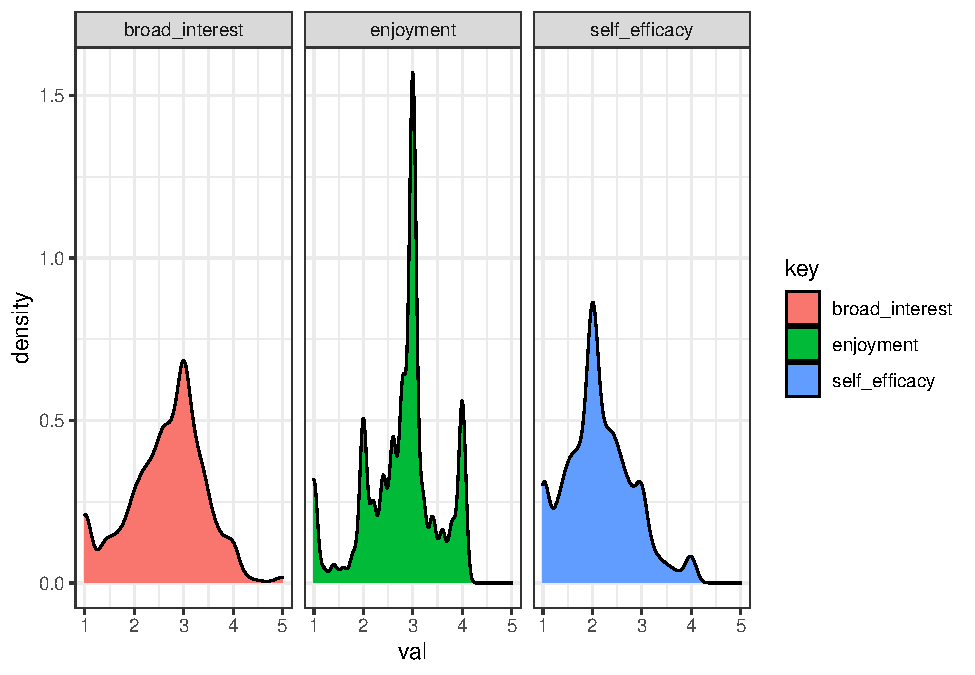
\includegraphics{paper_files/figure-latex/unnamed-chunk-6-1.pdf}
We see that the data broadly \emph{appears} to be normally distributed, as the following statistics from the use of the psych package suggest:

\begin{Shaded}
\begin{Highlighting}[]
\NormalTok{pisaUSA15 }\OperatorTok
\StringTok{  }\KeywordTok{select}\NormalTok{(broad_interest, enjoyment, self_efficacy) }\OperatorTok\StringTok{ }
\StringTok{  }\NormalTok{psych}\OperatorTok{::}\KeywordTok{describe}\NormalTok{()}
\end{Highlighting}
\end{Shaded}

\begin{verbatim}
##                vars    n mean   sd median trimmed  mad min max range  skew
## broad_interest    1 5454 2.65 0.78    2.8    2.68 0.59   1   5     4 -0.28
## enjoyment         2 5520 2.78 0.75    3.0    2.82 0.59   1   4     3 -0.51
## self_efficacy     3 5409 2.14 0.67    2.0    2.11 0.64   1   4     3  0.44
##                kurtosis   se
## broad_interest    -0.03 0.01
## enjoyment          0.17 0.01
## self_efficacy      0.07 0.01
\end{verbatim}

\hypertarget{using-tidylpa-directly-and-exclusively-within-r}{%
\subsection{Using tidyLPA directly and exclusively within R}\label{using-tidylpa-directly-and-exclusively-within-r}}

First, we show how to use tidyLPA within R---without any need to use or purchase MPlus.

In these examples, we pass the results of one function to the next by \emph{piping}
(using the \texttt{\%\textgreater{}\%} operator, loaded from the \texttt{dplyr} package). We pass the data to
a function that selects relevant variables, and then to \texttt{estimate\_profiles}.

A simple summary of the analysis is printed to the console. The resulting object
can be further passed down a pipeline to other functions, such as
\texttt{compare\_solutions}, \texttt{get\_data}, and \texttt{get\_fit}.

\begin{Shaded}
\begin{Highlighting}[]
\NormalTok{pisaUSA15 }\OperatorTok
\StringTok{  }\KeywordTok{select}\NormalTok{(broad_interest, enjoyment, self_efficacy) }\OperatorTok
\StringTok{  }\KeywordTok{single_imputation}\NormalTok{() }\OperatorTok
\StringTok{  }\KeywordTok{estimate_profiles}\NormalTok{(}\DecValTok{3}\NormalTok{)}
\end{Highlighting}
\end{Shaded}

\begin{verbatim}
## tidyLPA analysis using mclust: 
## 
##  Model Classes AIC      BIC      Entropy prob_min prob_max n_min n_max BLRT_p
##  1     3       34805.16 34898.27 0.74    0.75     0.94     0.16  0.67  0.01
\end{verbatim}

\hypertarget{using-tidylpa-to-estimate-models-efficiently-and-reproducibly-in-mplus}{%
\subsection{Using tidyLPA to estimate models efficiently and reproducibly in Mplus}\label{using-tidylpa-to-estimate-models-efficiently-and-reproducibly-in-mplus}}

We can use Mplus simply by changing the package argument for
\texttt{estimate\_profiles()} to \enquote{mplus} or \enquote{MplusAutomation} (either will work; not run
here):

\begin{Shaded}
\begin{Highlighting}[]
\NormalTok{pisaUSA15 }\OperatorTok
\StringTok{  }\KeywordTok{select}\NormalTok{(broad_interest, enjoyment, self_efficacy) }\OperatorTok
\StringTok{  }\KeywordTok{single_imputation}\NormalTok{() }\OperatorTok
\StringTok{  }\KeywordTok{estimate_profiles}\NormalTok{(}\DecValTok{3}\NormalTok{, }\DataTypeTok{package =} \StringTok{"mplus"}\NormalTok{)}
\end{Highlighting}
\end{Shaded}

\begin{verbatim}
## tidyLPA analysis using mplus: 
## 
##  Model Classes AIC      BIC      Entropy prob_min prob_max n_min n_max BLRT_p
##  1     3       34809.14 34902.24 0.77    0.79     0.94     0.16  0.67  0.00
\end{verbatim}

These are the very basics; we will return to what we do with this output later
in the tutorial.

\hypertarget{determining-the-fit-of-an-estimated-model}{%
\subsection{Determining the Fit of an Estimated Model}\label{determining-the-fit-of-an-estimated-model}}

We can see a number of statistics for each of the models that were estimated,
including the AIC (Aikake information criterion; based on -2 * the
log-likelihood, and penalized by number of parameters) and BIC (BIC: Bayesian
information criterion; based on -2 log-likelihood, and penalized by number of
parameters adjusted by sample size). Both are \emph{penalized} likelihood statistics;
the log-likelihood will always decrease with the addition of additional
paremeters estimated by the model, whereas the AIC and BIC will account for the
number of parameters; lower values of either indicate better fit.

Entropy. \texttt{prob\_min} refers to the minimum of the diagonal of the average latent
class probabilities for most likely class membership, by assigned class. The
minimum should be as high as possible, reflecting greater classification
certainty (cases are assigned to classes they have a high probability of
belonging to; see Jung \& Wickrama, 2008); \texttt{prob\_max} refers to the maximum.
Finally. \texttt{n\_min} refers to the proportion of the sample assigned to the smallest
class (based on most likely class membership); \texttt{n\_max} to the largest. Finally,
\texttt{BLRT\_p} refers to the p-value for the bootstrapped likelihood ratio test; a
value greater than .05 indicates that the model fit better than one with one
fewer class. Additional fit statistics (other penalized likelihood values, such
as the CAIC, SABIC, and ICL), and the bootstrapped LRT test statistic, can be
obtained with the \texttt{get\_fit()} function (processed with the tidyr R package to be in \enquote{long} rather than \enquote{wide} format):

\begin{Shaded}
\begin{Highlighting}[]
\KeywordTok{library}\NormalTok{(tidyr)}

\NormalTok{pisaUSA15 }\OperatorTok
\StringTok{  }\KeywordTok{select}\NormalTok{(broad_interest, enjoyment, self_efficacy) }\OperatorTok
\StringTok{  }\KeywordTok{single_imputation}\NormalTok{() }\OperatorTok
\StringTok{  }\KeywordTok{estimate_profiles}\NormalTok{(}\DecValTok{3}\NormalTok{) }\OperatorTok\StringTok{ }
\StringTok{  }\KeywordTok{get_fit}\NormalTok{(m1) }\OperatorTok\StringTok{ }
\StringTok{  }\KeywordTok{gather}\NormalTok{(stat, val)}
\end{Highlighting}
\end{Shaded}

\begin{verbatim}
## # A tibble: 18 x 2
##    stat              val
##    <chr>           <dbl>
##  1 Model         1      
##  2 Classes       3      
##  3 LogLik   -17399.     
##  4 AIC       34826.     
##  5 AWE       35080.     
##  6 BIC       34919.     
##  7 CAIC      34933.     
##  8 CLC       34799.     
##  9 KIC       34843.     
## 10 SABIC     34874.     
## 11 ICL      -36442.     
## 12 Entropy       0.744  
## 13 prob_min      0.750  
## 14 prob_max      0.936  
## 15 n_min         0.161  
## 16 n_max         0.669  
## 17 BLRT_val    649.     
## 18 BLRT_p        0.00990
\end{verbatim}

\hypertarget{comparing-the-fit-for-many-estimated-models}{%
\subsection{Comparing the Fit for Many Estimated Models}\label{comparing-the-fit-for-many-estimated-models}}

The function \texttt{compare\_solutions()} compares the fit of several estimated models,
with varying numbers of profiles and model specifications:

\begin{Shaded}
\begin{Highlighting}[]
\NormalTok{many_analyses_}\DecValTok{1}\NormalTok{_}\DecValTok{3}\NormalTok{ <-}\StringTok{ }\NormalTok{pisaUSA15 }\OperatorTok
\StringTok{  }\KeywordTok{select}\NormalTok{(broad_interest, enjoyment, self_efficacy) }\OperatorTok
\StringTok{  }\KeywordTok{single_imputation}\NormalTok{() }\OperatorTok
\StringTok{  }\KeywordTok{estimate_profiles}\NormalTok{(}\DataTypeTok{models =} \KeywordTok{c}\NormalTok{(}\DecValTok{1}\NormalTok{, }\DecValTok{3}\NormalTok{),}
                    \DataTypeTok{n_profiles =} \DecValTok{1}\OperatorTok{:}\DecValTok{5}\NormalTok{)}

\KeywordTok{compare_solutions}\NormalTok{(many_analyses_}\DecValTok{1}\NormalTok{_}\DecValTok{3}\NormalTok{)}
\end{Highlighting}
\end{Shaded}

\begin{verbatim}
## Compare tidyLPA solutions:
## 
##  Model Classes BIC      Warnings
##  1     1       38089.12         
##  1     2       35632.66         
##  1     3       34991.63         
##  1     4       33145.73         
##  1     5       32830.99         
##  3     1       35262.73         
##  3     2       34836.77         
##  3     3       34868.19         
##  3     4       34600.33 Warning 
##  3     5       34391.97         
## 
## Best model according to BIC is Model 1 with 5 classes.
## 
## An analytic hierarchy process, based on the fit indices AIC, AWE, BIC, CLC, and KIC (Akogul & Erisoglu, 2017), suggests the best solution is Model 1 with 5 classes.
\end{verbatim}

\hypertarget{inspecting-and-plotting-the-best-fitting-estimated-models}{%
\subsection{Inspecting and Plotting the best-fitting estimated models}\label{inspecting-and-plotting-the-best-fitting-estimated-models}}

It appears that the four and five-class solutions fit best. Let's inspect those, specifically:

\begin{Shaded}
\begin{Highlighting}[]
\NormalTok{models_}\DecValTok{4}\NormalTok{_}\DecValTok{5}\NormalTok{ <-}\StringTok{ }\NormalTok{pisaUSA15[}\DecValTok{1}\OperatorTok{:}\DecValTok{100}\NormalTok{, ] }\OperatorTok
\StringTok{  }\KeywordTok{select}\NormalTok{(broad_interest, enjoyment, self_efficacy) }\OperatorTok
\StringTok{  }\KeywordTok{single_imputation}\NormalTok{() }\OperatorTok
\StringTok{  }\KeywordTok{estimate_profiles}\NormalTok{(}\DataTypeTok{models =} \DecValTok{1}\NormalTok{,}
                    \DataTypeTok{n_profiles =} \KeywordTok{c}\NormalTok{(}\DecValTok{4}\NormalTok{, }\DecValTok{5}\NormalTok{))}

\NormalTok{models_}\DecValTok{4}\NormalTok{_}\DecValTok{5} \OperatorTok\StringTok{ }
\StringTok{  }\KeywordTok{plot_profiles}\NormalTok{(}\DataTypeTok{add_line =} \OtherTok{TRUE}\NormalTok{)}
\end{Highlighting}
\end{Shaded}

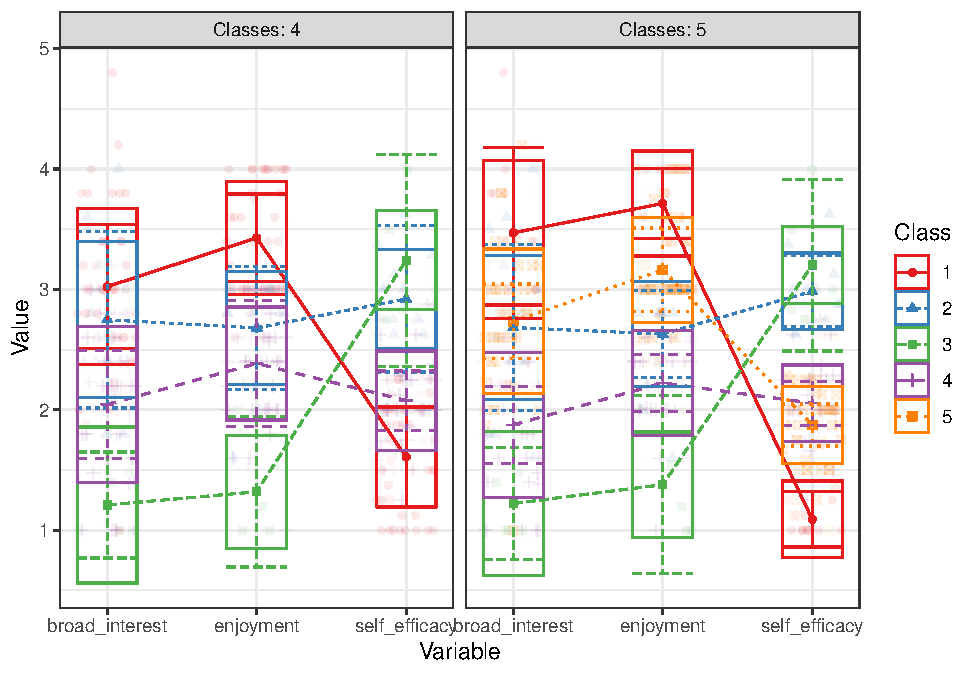
\includegraphics{paper_files/figure-latex/unnamed-chunk-8-1.pdf}

Here, it appears that the addition of a fifth class does not add a great deal relative to the four-class solution. Accordingly, we consider the four-class solution to be the solution we interpret and present, while heeding the recommendations about reporting which other models we estimated, how we chose to focus on the two best-fitting models we did, and why we presented the four-class, class-invariant set of estimates.

Were we to wish to inspect \emph{only} that chosen model, we could estimate the model again, replacing \texttt{n\_profiles\ =\ c(4,\ 5)} with \texttt{n\_profiles\ =\ 4}. Alternatively, we could use list-indexing within R to index only that model. Note that the object \texttt{models\_4\_5} below includes the four and five-class estimated models, in that order. Using \texttt{{[}{[}1{]}{]}} indexes---selects---only the first of the two models, whereas \texttt{{[}{[}2{]}{]}} indexes the second. We index the four-class solution using \texttt{{[}{[}1{]}{]}}, and save it to a new object.

Using this single estimated model, we can also create a faceted plot of density plots for an object of class \enquote{tidyLPA}. For each variable, a Total density plot will be shown, where cases are weighted by the posterior probability of being assigned to that class:

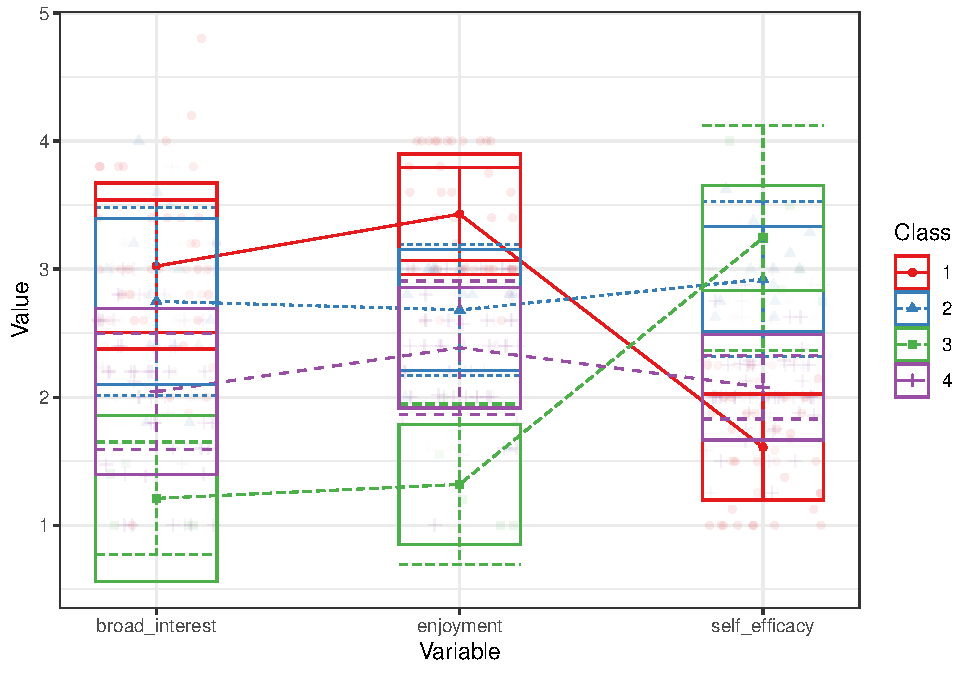
\includegraphics{paper_files/figure-latex/unnamed-chunk-10-1.pdf}

\hypertarget{visualizing-and-examining-a-chosen-solution-further}{%
\subsection{Visualizing and Examining a Chosen Solution Further}\label{visualizing-and-examining-a-chosen-solution-further}}

Last, we can create a faceted plot of two-dimensional correlation plots and unidimensional density plots for a single set of model estimates:
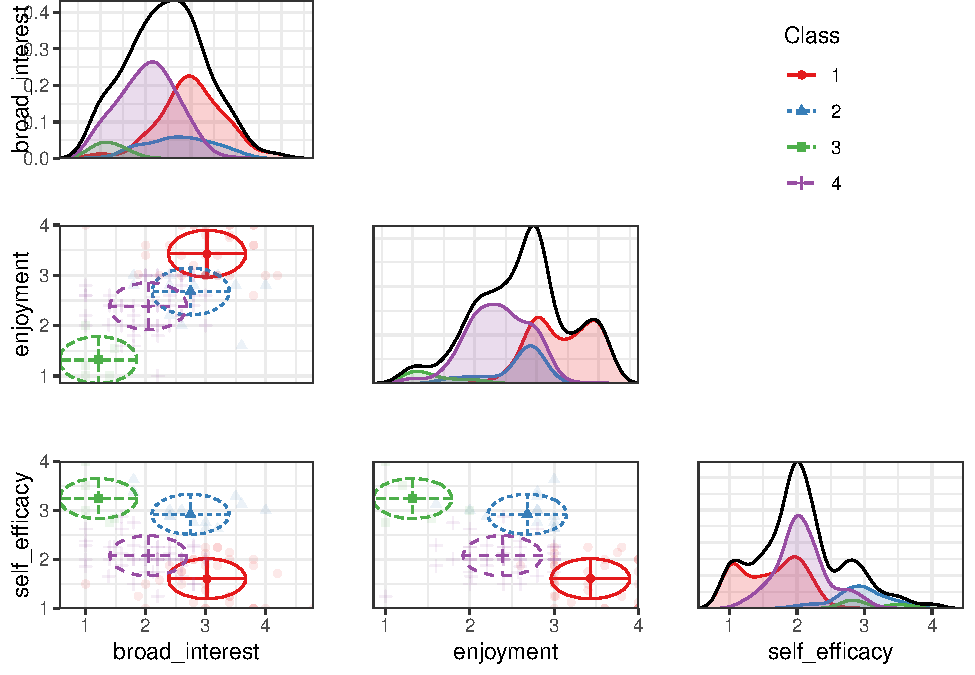
\includegraphics{paper_files/figure-latex/unnamed-chunk-11-1.pdf}
We can use \texttt{get\_data()} to return data in wide format when applied to an object
of class tidyProfile (one element of a tidyLPA object)

\texttt{get\_data()} returns long format when applied to a
tidyLPA object containing multiple tidyProfile analyses (because then the wide
format does not make sense).

To transform data in the wide format into the long format, the \texttt{gather()}
function from the \textbf{tidyr} package can be used:

\begin{Shaded}
\begin{Highlighting}[]
\KeywordTok{get_data}\NormalTok{(model_}\DecValTok{4}\NormalTok{) }\OperatorTok\StringTok{ }
\StringTok{  }\NormalTok{tidyr}\OperatorTok{::}\KeywordTok{gather}\NormalTok{(Class_prob, Probability, }\KeywordTok{contains}\NormalTok{(}\StringTok{"CPROB"}\NormalTok{))}
\end{Highlighting}
\end{Shaded}

\begin{verbatim}
## # A tibble: 400 x 8
##    model_number classes_number broad_interest enjoyment self_efficacy Class
##           <dbl>          <dbl>          <dbl>     <dbl>         <dbl> <dbl>
##  1            1              4            3.8       4            1        1
##  2            1              4            3         3            2.75     2
##  3            1              4            1.8       2.8          3.38     2
##  4            1              4            1.4       1            2.75     3
##  5            1              4            1.8       2.2          2        4
##  6            1              4            1.6       1.6          1.88     4
##  7            1              4            3         3.8          2.25     1
##  8            1              4            2.6       2.2          2        4
##  9            1              4            1         2.8          2.62     4
## 10            1              4            2.2       2            1.75     4
## # ... with 390 more rows, and 2 more variables: Class_prob <chr>,
## #   Probability <dbl>
\end{verbatim}

\hypertarget{best-practices-for-latent-profile-analysis}{%
\section{Best Practices for Latent Profile Analysis}\label{best-practices-for-latent-profile-analysis}}

In addition to the pragmatic challenges facing the analyst carrying out LPA, there
are a number of statistical issues that anaylsts face. Past research is informative in
this respect; Bauer

\hypertarget{recommendations-regarding-analytic-choices}{%
\subsection{Recommendations Regarding Analytic Choices}\label{recommendations-regarding-analytic-choices}}

A note of caution is warranted about LPA in the context of their characteristics
and strengths. Bauer (2007) notes that many samples of data can be usefully
broken down into profiles, and that the addition of profiles will likely be
suggested for reasons other than the samples coming from more than one
distribution (i.e., due to non-normality in the variables measured). Bauer also
cautions that profiles should not be reified; that profiles do not necessarily
exist outside of the analysis that they should be interpreted more as useful
interpretative devices. These cautions suggest that, in general, parsimony,
interpretability, and a general sense that the profiles are not necessarily
real, but are rather helpful analytic tools, should be both priorities for the
analyst and the reader of studies using this approach.

The GRoLTs checklist, developed for a particular use of the general mixture
model---a growth mixture model---is a helpful way to think about how best
practices for LPA (Van De Schoot, Sijbrandij, Winter, Depaoli, \& Vermunt, 2017). We interpret them in light of LPA; note that
the full checklist is not applicable (as, for example, guidelines about
trajectories over time are not pertinent to LPA), and we only present those that
are.

First, here is the checklist:

\hypertarget{grolts-checklist}{%
\subsection{GRoLTs checklist}\label{grolts-checklist}}

\hypertarget{htmlwidget-fffc7926638efd89a6a8}{}

We walk through each of these in turn.

\hypertarget{is-the-missing-data-mechanism-reported}{%
\subsubsection{Is the missing data mechanism reported?}\label{is-the-missing-data-mechanism-reported}}

As missing data can have a bearing on the estimates, an important consideration is whether or not the missing data is associated with the levels of the variables---or not. Consider consulting general guidelines on missing data, including Enders (2010), Little \& Rubin (2019), and Allison (2001).
\#\#\# Is a description provided of what variables are related to attrition/missing data?

Note whether any demographic or other variables are related to missing data.

\hypertarget{is-a-description-provided-of-how-missing-data-in-the-analyses-were-dealt-with}{%
\subsubsection{Is a description provided of how missing data in the analyses were dealt with?}\label{is-a-description-provided-of-how-missing-data-in-the-analyses-were-dealt-with}}

Because LPA cannot accomodate any missing values (and so uses listwise deletion) for this recommendation, tidyLPA has a function for addressing missing data that are based upon single imputation (with two methods available, one using a contemporary, machine learning-based procedure).

\hypertarget{is-information-about-the-distribution-of-the-observed-variables-included}{%
\subsubsection{Is information about the distribution of the observed variables included?}\label{is-information-about-the-distribution-of-the-observed-variables-included}}

The variables can be plotted and described prior to the analyses. While not built-in, we show later how this can be done using the ggplot2 R package, and the \texttt{describe()} function from the psych R package.

\hypertarget{is-the-software-mentioned}{%
\subsubsection{Is the software mentioned?}\label{is-the-software-mentioned}}

The name and version of the software can be mentioned. Within R, a citation including the version can be generated for any R package, including tidyLPA, by using the \texttt{citation()} function (e.g., `citation(\enquote{tidyLPA})).

\hypertarget{are-alternative-specifications-of-the-between-class-differences-in-variancecovariance-matrix-structure-considered-and-clearly-documented}{%
\subsubsection{Are alternative specifications of the between-class differences in variance--covariance matrix structure considered and clearly documented?}\label{are-alternative-specifications-of-the-between-class-differences-in-variancecovariance-matrix-structure-considered-and-clearly-documented}}

In LPA, we can determine which parameters - variance and covariance - are
estimated to be the same or different across all profiles, and, in the case of
covariance, whether it is fixed to zero. Of course, for the profiles we are most
interested in, the mean is allowed to vary across profiles.

In general, the approach to choosing the model is similar to choosing the number
of profiles, requiring \textbf{deciding on the basis of evidence from multiple
sources}, including information criteria, statistical tests, and concerns of
interpretability and parsimony. The article by \href{https://www.sciencedirect.com/science/article/pii/S0361476X06000543}{Pastor and colleagues
(2007)} has
helpful information on the model specifications.

Here, the six models that are possible to specify in LPA are described in terms of how the variables used to create the profiles are estimated. In tidyLPA, the models are specified by passing
arguments to the \texttt{variance} and \texttt{covariance} arguments. The possible values for
these arguments are:

\begin{itemize}
\tightlist
\item
  \texttt{variances}: \enquote{equal} and \enquote{zero}
\item
  \texttt{covariances}: \enquote{varying}, \enquote{equal}, and \enquote{zero}
\end{itemize}

These models are described in Appendix A.

\hypertarget{is-information-reported-about-the-number-of-random-start-values-and-final-iterations-included}{%
\subsubsection{Is information reported about the number of random start values and final iterations included?}\label{is-information-reported-about-the-number-of-random-start-values-and-final-iterations-included}}

MPlus uses random starts to initialize the estimation, whereas mclust (the R package) does not. Thus, for users of MPlus, the number of random starts and final iterations should be reported. By default, tidyLPA uses the MPlus defaults. Information on the number of random starts can be found in the model object returned by the tidyLPA function \texttt{estimate\_profiles()}. Different random starts can be passed by passing arguments to the \texttt{ANALYSIS} code for MPlus, e.g.:

\hypertarget{are-the-model-comparison-and-selection-tools-described-from-a-statistical-perspective}{%
\subsubsection{Are the model comparison (and selection) tools described from a statistical perspective?}\label{are-the-model-comparison-and-selection-tools-described-from-a-statistical-perspective}}

In the case of choosing the number of profiles (and the specification of the
model / profile solution), multiple criteria, such as the BIC or the proportion
of variance explained are recommended for decision-making, but also
interpretability in light of theory, parsimony, and evidence from
cross-validation should be considered.

We provide a number of functions for model comparison. The \texttt{compare\_solutions()} profile
takes as an argument a particular measure of fit (defaulting to the BIC), and returns information
for all of the models estimated. It also implements an ensemble, analytic hierarchiy approach, that uses weighted values of a number of fit indices; see (Akogul \& Erisoglu, 2017) for more.

\hypertarget{are-the-total-number-of-fitted-models-reported-including-a-one-class-solution}{%
\subsubsection{Are the total number of fitted models reported, including a one-class solution?}\label{are-the-total-number-of-fitted-models-reported-including-a-one-class-solution}}

The number of fitted models can easily be reported based on the tidyLPA code run. For example, for the following code, models with 1-6 profiles, and the first (class invariant) and third (class invariant, unrestricted) model parameterizations are estimated:

\hypertarget{are-the-number-of-cases-per-class-reported-for-each-model-absolute-sample-size-or-proportion}{%
\subsubsection{Are the number of cases per class reported for each model (absolute sample size, or proportion)?}\label{are-the-number-of-cases-per-class-reported-for-each-model-absolute-sample-size-or-proportion}}

Determining the number of cases per class can easily be done by using the \texttt{get\_data()} function from tidyLPA, passing the estimated model object from tidyLPA.; see the \texttt{Class} column (as well as the posterior probability estimates for every class for every observation).

\hypertarget{are-all-of-the-estimates-plotted}{%
\subsubsection{Are all of the estimates plotted?}\label{are-all-of-the-estimates-plotted}}

This is a recommendation which can be difficult to achieve using existing software. tidyLPA provides two functions, \texttt{plot\_profiles()} and \texttt{plot\_bivariate()}, to plot the estimates.

\hypertarget{are-the-raw-data-plotted-along-with-the-estimates}{%
\subsubsection{Are the raw data plotted along with the estimates?}\label{are-the-raw-data-plotted-along-with-the-estimates}}

The above-mentioned tidyLPA functions also plot the raw data with the estimates (by default).

\hypertarget{are-characteristics-of-the-final-class-solution-numerically-described-i.e.-means-sdse-n-ci-etc.}{%
\subsubsection{Are characteristics of the final class solution numerically described (i.e., means, SD/SE, n, CI, etc.)?}\label{are-characteristics-of-the-final-class-solution-numerically-described-i.e.-means-sdse-n-ci-etc.}}

These characteristics can be obtained by using the \texttt{get\_estimates()} function, passing the estimated model object from tidyLPA.

\hypertarget{are-the-syntax-files-available-either-in-the-appendix-supplementary-materials-or-from-the-authors}{%
\subsubsection{Are the syntax files available (either in the appendix, supplementary materials, or from the authors)?}\label{are-the-syntax-files-available-either-in-the-appendix-supplementary-materials-or-from-the-authors}}

The R files used for the analyses can easily be included in online repositories and supplementary online materials (as \texttt{.R} or \texttt{.Rmd} files).

\hypertarget{summary-and-conclusion}{%
\section{Summary and Conclusion}\label{summary-and-conclusion}}

A step away from the tutorial side of this work, we wish to note some
implications for the developers of statistical software for psychological
scientists.

First, we note that developing a tool that emphasized both rigor and access has
been, so far, well-received. This suggests that there is an audience (or a
market) for tools to carry out sophisticated tools that may be otherwise
out-of-reach. Tools do not need to be hard to use, a point made by developers
of, for example, tools to carry out highly-sophisticated Bayesian methods using
the most cutting-edge tools (Bürkner \& others, 2017, Makowski, Ben-Shachar, Chen, and Lüdecke (2019)). We think that
tidyLPA speaks to this, too.

Another implication concerns how we developed tidyLPA. We used a modern software
development workflow, including git/GitHub, a suite of tests, and continuous
integration tools. We also note that we emphasized communicating that we were
developing the software; when it was updated; and how we made major updates.

There are a number of analytic choices that need to be made when carrying out
person-oriented analyses. Because such person-oriented approaches are often more
subjective (in practice) than other approaches (Linnenbrink-Garcia and
Wormington, 2017), there is no one rule for determining the solution obtained.
This solution is obtained on the basis of multiple decisions, such as the number
of profiles selected or the modeling decisions such as what specific options are
used for the cluster analysis (i.e., the distance metric used to calculate the
similarity of the observations as part of the Ward's hierarchical clustering) or
what parameters are estimated and how as part of LPA.

Given the subjectivity involved, it is important that researchers be transparent
and work as part of a team to obtain clustering solutions. Transparency about
the design and analytic choices is important so that readers can appropriately
interpret the report. Researchers can enhance transparency and reproducibility
by sharing detailed descriptions of methodology and document it through the use
of syntax (and, if possible, data) that we share with others. Working as part of
a team can help to serve as a check on several of the choices researchers make,
such as over-fitting or under-fitting the model to the data. Each decision
depends on multiple factors and balancing tensions. We discuss each of the key
decisions listed in an analysis.

LPA can be used to evaluate how psychological constructs are experienced (and
can be analyzed) together and at once. Though described in contrast to a
variable-centered approach, scholars have pointed out how person-oriented
approaches, including LPA, are complementary to variable-centered analyses
(Marsh, Ludtke, Trautwein, \& Morin, 2009). Our aim was to describe how
researchers may get started in an informed way as researchers seek to understand
how individuals interact, behave, and learn in ways that embraces the complexity
of these experiences.

\hypertarget{appendix-a}{%
\section{Appendix A}\label{appendix-a}}

Note that \emph{p} represents different profiles and each parameterization is represented by a 4 x 4 covariance matrix and therefore would represent the parameterization for a four-profile solution. In all of the models, the means are estimated freely in the different profiles. Imagine that each row and column represents a different variable, i.e., the first row (and column) represents broad interest, the second enjoyment, the third self-efficacy, and the fourth another variable, i.e., future goals and plans.

\hypertarget{equal-variances-and-covariances-fixed-to-0-model-1}{%
\subsubsection{1. Equal variances, and covariances fixed to 0 (model 1)}\label{equal-variances-and-covariances-fixed-to-0-model-1}}

In this model, which corresponds to the mclust model wit the name \enquote{EEI}, the variances are estimated to be equal across profiles, indicated by the absence of a p subscript for any of the diagonal elements of the matrix. The covariances are constrained to be zero, as indicated by the 0's between every combination of the variables.

It is specified with \texttt{variances\ =\ "equal"} and \texttt{covariances\ =\ "zero"}.

This model is highly constrained but also parsimonious: the profiles are estimated in such a way that the variables' variances are identical for each of the profiles, and the relationships between the variables are not estimated. In this way, less degrees of freedom are taken used to explain the observations that make up the data. However, estimating more parameters--as in the other models--may better explain the data, justifying the addition in complexity that their addition involves (and their reduction in degrees of freedom). This model is sometimes referred to as a \emph{class-invariant} parameterization.

\[
\left[ \begin{matrix} { \sigma  }_{ 1 }^{ 2 } & 0 & 0 & 0 \\ 0 & { \sigma  }_{ 2 }^{ 2 } & 0 & 0 \\ 0 & 0 & { \sigma  }_{ 3 }^{ 2 } & 0 \\ 0 & 0 & 0 & { \sigma  }_{ 4 }^{ 2 } \end{matrix} \right] 
\]

\hypertarget{varying-variances-and-covariances-fixed-to-0-model-2}{%
\subsubsection{2. Varying variances and covariances fixed to 0 (model 2)}\label{varying-variances-and-covariances-fixed-to-0-model-2}}

This model corresponds to the mclust model \enquote{VVI} and allows for the variances to be freely estimated across profiles. The covariances are constrained to zero.

It is specified with \texttt{variances\ =\ "varying"} and \texttt{covariances\ =\ "zero"}.

Thus, it is more flexible (and less parsimonious) than model 1, but in terms of the covariances, is more constrained than model 2. This model is sometimes referred to as a \emph{class-varying diagonal} parameterization.

\[ 
\left[ \begin{matrix} { \sigma  }_{ 1p }^{ 2 } & 0 & 0 & 0 \\ 0 & { \sigma  }_{ 2p }^{ 2 } & 0 & 0 \\ 0 & 0 & { \sigma  }_{ 3p }^{ 2 } & 0 \\ 0 & 0 & 0 & { \sigma  }_{ 4p }^{ 2 } \end{matrix} \right] 
\]

\hypertarget{equal-variances-and-equal-covariances-model-3}{%
\subsubsection{3. Equal variances and equal covariances (model 3)}\label{equal-variances-and-equal-covariances-model-3}}

This model corresponds to the mclust model \enquote{EEE}. In this model, the variances are still constrained to be the same across the profiles, although now the covariances are estimated (but like the variances, are constrained to be the same across profiles).

It is specified with \texttt{variances\ =\ "equal"} and \texttt{covariances\ =\ "equal"}.

Thus, this model is the first to estimate the covariance (or correlations) of the variables used to create the profiles, thus adding more information that can be used to better understand the characteristics of the profiles (and, potentially, better explain the data). This model is sometimes referred to as a \emph{class-invariant unrestricted} parameterization.

\[
\left[ \begin{matrix} { \sigma  }_{ 1 }^{ 2 } & { \sigma  }_{ 21 } & { \sigma  }_{ 31 } & { \sigma  }_{ 41 } \\ { \sigma  }_{ 12 } & { \sigma  }_{ 2 }^{ 2 } & { \sigma  }_{ 23 } & { \sigma  }_{ 24 } \\ { \sigma  }_{ 13 } & { \sigma  }_{ 12 } & { \sigma  }_{ 3 }^{ 2 } & { \sigma  }_{ 33 } \\ { \sigma  }_{ 14 } & { \sigma  }_{ 12 } & { \sigma  }_{ 12 } & { \sigma  }_{ 4 }^{ 2 } \end{matrix} \right] 
\]

\hypertarget{varying-means-varying-variances-and-equal-covariances-model-4}{%
\subsubsection{4. Varying means, varying variances, and equal covariances (model 4)}\label{varying-means-varying-variances-and-equal-covariances-model-4}}

This model, which specifies for the variances to be freely estimated across the profiles and for the covariances to be estimated to be equal across profiles, extends model 3.

It is specified with \texttt{variances\ =\ "varying"} and \texttt{covariances\ =\ "equal"}.

Unfortunately, this model cannot be specified with mclust, though it can be with MPlus; this model \emph{can} be used with the functions to interface to MPlus described below.

\[
\left[ \begin{matrix} { \sigma  }_{ 1p }^{ 2 } & { \sigma  }_{ 21 } & { \sigma  }_{ 31 } & { \sigma  }_{ 41 } \\ { \sigma  }_{ 12 } & { \sigma  }_{ 2p }^{ 2 } & { \sigma  }_{ 23 } & { \sigma  }_{ 24 } \\ { \sigma  }_{ 13 } & { \sigma  }_{ 12 } & { \sigma  }_{ 3p }^{ 2 } & { \sigma  }_{ 33 } \\ { \sigma  }_{ 14 } & { \sigma  }_{ 12 } & { \sigma  }_{ 12 } & { \sigma  }_{ 4p }^{ 2 } \end{matrix} \right] 
\]

\hypertarget{varying-means-equal-variances-and-varying-covariances-model-5}{%
\subsubsection{5. Varying means, equal variances, and varying covariances (model 5)}\label{varying-means-equal-variances-and-varying-covariances-model-5}}

This model specifies the variances to be equal across the profiles, but allows the covariances to be freely estimated across the profiles.

It is specified with \texttt{variances\ =\ "equal"} and \texttt{covariances\ =\ "varying"}.

Like model 4, this model cannot be specified with mclust, though it can be with MPlus. Again, this model \emph{can} be used with the functions to interface to MPlus described below.

\[
\left[ \begin{matrix} { \sigma  }_{ 1 }^{ 2 } & { \sigma  }_{ 21p } & { \sigma  }_{ 31p } & { \sigma  }_{ 41p } \\ { \sigma  }_{ 12p } & { \sigma  }_{ 2 }^{ 2 } & { \sigma  }_{ 23p } & { \sigma  }_{ 24p } \\ { \sigma  }_{ 13p } & { \sigma  }_{ 12p } & { \sigma  }_{ 3 }^{ 2 } & { \sigma  }_{ 33p } \\ { \sigma  }_{ 14p } & { \sigma  }_{ 12p } & { \sigma  }_{ 12p } & { \sigma  }_{ 4 }^{ 2 } \end{matrix} \right] \quad 
\]

\hypertarget{varying-variances-and-varying-covariances-model-6}{%
\subsubsection{6. Varying variances and varying covariances (model 6)}\label{varying-variances-and-varying-covariances-model-6}}

This model corresponds to the mclust model \enquote{VVV}. It allows the variances and the covariances to be freely estimated across profiles.

It is specified with \texttt{variances\ =\ "varying"} and \texttt{covariances\ =\ "varying"}.

Thus, it is the most complex model, with the potential to allow for understanding many aspects of the variables that are used to estimate the profiles and how they are related. However, it is less parsimonious than all of the other models, and the added parameters should be considered in light of how preferred this model is relative to those with more simple specifications. This model is sometimes referred to as a \emph{class-varying unrestricted} parameterization.

\[
\left[ \begin{matrix} { \sigma  }_{ 1p }^{ 2 } & { \sigma  }_{ 21p } & { \sigma  }_{ 31p } & { \sigma  }_{ 41p } \\ { \sigma  }_{ 12p } & { \sigma  }_{ 2p }^{ 2 } & { \sigma  }_{ 23p } & { \sigma  }_{ 24p } \\ { \sigma  }_{ 13p } & { \sigma  }_{ 12p } & { \sigma  }_{ 3p }^{ 2 } & { \sigma  }_{ 33p } \\ { \sigma  }_{ 14p } & { \sigma  }_{ 12p } & { \sigma  }_{ 12p } & { \sigma  }_{ 4p }^{ 2 } \end{matrix} \right] 
\]

\hypertarget{references}{%
\section{References}\label{references}}

\begingroup
\setlength{\parindent}{-0.5in}
\setlength{\leftskip}{0.5in}

\hypertarget{refs}{}
\leavevmode\hypertarget{ref-akogul2017approach}{}%
Akogul, S., \& Erisoglu, M. (2017). An approach for determining the number of clusters in a model-based cluster analysis. \emph{Entropy}, \emph{19}(9), 452.

\leavevmode\hypertarget{ref-allison2001missing}{}%
Allison, P. D. (2001). \emph{Missing data} (Vol. 136). Sage publications.

\leavevmode\hypertarget{ref-burkner2017}{}%
Bürkner, P.-C., \& others. (2017). Brms: An r package for bayesian multilevel models using stan. \emph{Journal of Statistical Software}, \emph{80}(1), 1--28.

\leavevmode\hypertarget{ref-enders2010applied}{}%
Enders, C. K. (2010). \emph{Applied missing data analysis}. Guilford press.

\leavevmode\hypertarget{ref-little2019statistical}{}%
Little, R. J., \& Rubin, D. B. (2019). \emph{Statistical analysis with missing data} (Vol. 793). John Wiley \& Sons.

\leavevmode\hypertarget{ref-makowski2019}{}%
Makowski, D., Ben-Shachar, M. S., Chen, S., \& Lüdecke, D. (2019). Indices of effect existence and significance in the bayesian framework. \emph{Frontiers in Psychology}, \emph{10}, 2767.

\leavevmode\hypertarget{ref-R-tidyLPA}{}%
Rosenberg, J. M., Beymer, P. N., Anderson, D. J., Lissa, C. van, \& Schmidt, J. A. (2018). TidyLPA: An r package to easily carry out latent profile analysis (lpa) using open-source or commercial software. \emph{Journal of Open Source Software}, \emph{3}(30), 978. doi:\href{https://doi.org/10.21105/joss.00978}{10.21105/joss.00978}

\leavevmode\hypertarget{ref-van2017grolts}{}%
Van De Schoot, R., Sijbrandij, M., Winter, S. D., Depaoli, S., \& Vermunt, J. K. (2017). The grolts-checklist: Guidelines for reporting on latent trajectory studies. \emph{Structural Equation Modeling: A Multidisciplinary Journal}, \emph{24}(3), 451--467.

\leavevmode\hypertarget{ref-akogul2017approach}{}%
Akogul, S., \& Erisoglu, M. (2017). An approach for determining the number of clusters in a model-based cluster analysis. \emph{Entropy}, \emph{19}(9), 452.

\leavevmode\hypertarget{ref-allison2001missing}{}%
Allison, P. D. (2001). \emph{Missing data} (Vol. 136). Sage publications.

\leavevmode\hypertarget{ref-burkner2017}{}%
Bürkner, P.-C., \& others. (2017). Brms: An r package for bayesian multilevel models using stan. \emph{Journal of Statistical Software}, \emph{80}(1), 1--28.

\leavevmode\hypertarget{ref-enders2010applied}{}%
Enders, C. K. (2010). \emph{Applied missing data analysis}. Guilford press.

\leavevmode\hypertarget{ref-little2019statistical}{}%
Little, R. J., \& Rubin, D. B. (2019). \emph{Statistical analysis with missing data} (Vol. 793). John Wiley \& Sons.

\leavevmode\hypertarget{ref-makowski2019}{}%
Makowski, D., Ben-Shachar, M. S., Chen, S., \& Lüdecke, D. (2019). Indices of effect existence and significance in the bayesian framework. \emph{Frontiers in Psychology}, \emph{10}, 2767.

\leavevmode\hypertarget{ref-R-tidyLPA}{}%
Rosenberg, J. M., Beymer, P. N., Anderson, D. J., Lissa, C. van, \& Schmidt, J. A. (2018). TidyLPA: An r package to easily carry out latent profile analysis (lpa) using open-source or commercial software. \emph{Journal of Open Source Software}, \emph{3}(30), 978. doi:\href{https://doi.org/10.21105/joss.00978}{10.21105/joss.00978}

\leavevmode\hypertarget{ref-van2017grolts}{}%
Van De Schoot, R., Sijbrandij, M., Winter, S. D., Depaoli, S., \& Vermunt, J. K. (2017). The grolts-checklist: Guidelines for reporting on latent trajectory studies. \emph{Structural Equation Modeling: A Multidisciplinary Journal}, \emph{24}(3), 451--467.

\endgroup

\end{document}
